% Copyright (C) 2010 Thomas L. Kula
% All Rights Reserved
%
% See the file LICENSE for license terms.
\documentclass[12pt]{article}
\usepackage{graphicx}
\usepackage{rotating}
\usepackage{fix-cm}
\setlength{\paperwidth}{5.5in}
\setlength{\paperheight}{8.5in}
\setlength{\textheight}{7.45in}
\setlength{\topmargin}{-1.0in}
\setlength{\oddsidemargin}{-0.5in}
\setlength{\evensidemargin}{-0.5in}
\setlength{\textwidth}{4.0in}
\setlength{\parindent}{0in}
\setlength{\parskip}{3mm}
\usepackage[print]{booklet} \nofiles
\source{\magstep0}{5.5in}{8.5in}
\target{\magstep0}{11in}{8.5in}
\setpdftargetpages
\pagestyle{empty}
\begin{document}


\begin{center}
{\fontsize{36}{48}\selectfont \textsc{Haiku a Day }}
\end{center}

\vspace*{3.5cm}

{\fontsize{26}{52}\selectfont 
With too much to do
	 
Time passes by too quickly
	 
And no time to stop

}

\vspace*{5.0cm}
\begin{center}
{\large{Issue 55: January 2010}} \\[5mm]
{\fontsize{8}{8}\selectfont  \textsc{ St. Joshua Norton Press }} \\[1mm]
{\fontsize{6}{6}\selectfont Mathom House in Midtown \textbar The People's Republic of Ames }
\end{center}


\newpage

Where the hell has February gone?

--- Thomas

http://kula.tproa.net/had/ \\
kula@tproa.net

Download this and previous HADs at the website, so you can
print out your own (DIY, yeah!) or if you want me to send
you one, send me your address, and maybe a stamp if you
are feeling nice. Or send me something you've made ---
trades always appreciated, postcards are nice too.

\vspace*{2cm}

1 January 2010

Start the year quiet \\
A pot of tea, a warm robe \\
Music plays softly

2 January 2010

The wind, blustery \\
A brisk walk on a cold day \\
Hot coffee restores

3 January 2010

Last vacation day \\
It's worse than actual work \\
Since work looms ahead

\newpage

4 January 2010

Inside, there is warmth \\
In the dark, a ray of light \\
The kitchen is cheer

5 Janaury 2010

For a task at hand \\
There exists no better way \\
Just wait, tomorrow

6 January 2010

When water comes near \\
Flour stirred becomes stretchy \\
Gluten makes good bread

7 Janaury 2010

Hello to you, Sun \\
Oh why must you bother me? \\
I just want to sleep

8 January 2010

Late night, early morn \\
Not a good combination \\
Tea will save me now

9 January 2010

I see clouds, racing \\
Blast across the sky, purple \\
In the setting Sun

10 January 2010

A cave, not of stone \\
Layers of blankets form this \\
Shelter of sweet sleep



\newpage

11 January 2010

Liquid not flowing \\
Hard to the touch, shattering \\
Push it and it breaks

12 January 2010

Hole in the bucket \\
Making it hard to fill up \\
Leaking on my shoes

13 January 2010

From whence do you hail? \\
This mere electron, screaming \\
To the ground it goes

14 January 2010

Quickly the weekend \\
Aproaches, looming nearer \\
Work receeding, goes

15 January 2010

Once written, now test \\
Will a weekend of pounding \\
Make it stand or fail?

16 January 2010

Instead of cleaning \\
I go out to a movie \\
It is much more fun

17 January 2010

Long, green and stringy \\
Celery looms in my mind \\
A guest strangely there

\newpage

18 January 2010

A tune unbidden \\
Music rumbling in my ears \\
Mind's inner soundtrack

19 January 2010

Pedalling quickly \\
Trying hard to go nowhere \\
As fast as they can

20 January 2010

A warm fuzzy cave \\
Invaded by a small draft \\
Blankets fall, I wake

21 January 2010

Electrons pushing \\
A gas, excited it glows \\
When bent, words outlined

22 January 2010

The horn toot of God \\
A sad anemic fog horn \\
Sound designer fail

23 January 2010

Small French presses gone \\
So a large French press is used. \\
More tea fine with me 

24 January 2010

Rain falls where snow was \\
Snow vainly stands, then dissolves \\
Wet ground uncaring


\newpage

25 January 2010

Fan spins noisily \\
As an ersatz clothes dryer \\
Water falls away

26 January 2010

Grinding makes pressure \\
My eyes wanting to pop out \\
Go away headache

27 January 2010

When testing is done \\
More problems reveal themselves \\
Scream, sigh, debug, code

28 January 2010

Ribbon torn, falling \\
A bookmark disintegrates \\
Just dust on the floor

29 January 2010

Uneasy quiet \\
The pager calm for how long \\
Make it to monday?

30 January 2010

A day of gumption \\
Ripped to shred by a pager \\
No love, macc-lib-1

31 January 2010

Sweet fanny Jebus \\
The tape slots have gone away \\
Order is restored


\newpage

\begin{center}
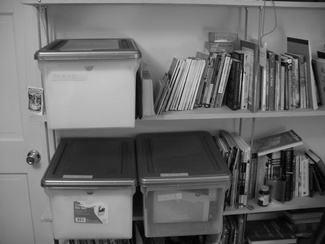
\includegraphics{happy-zines.jpg} \\[1cm]
Happiness is organized zines
\end{center}

\newpage

\thispagestyle{empty}
\vspace*{14cm}
\begin{sideways}
\Large{Thomas L. Kula}
\end{sideways}
\begin{sideways}
\Large{PO Box 980461}
\end{sideways}
\begin{sideways}
\Large{Ypsilanti MI 48198}
\end{sideways}


\end{document}


